% (c) 2012 Silvia Cibola - silvia.cibola@gmail.com
% (c) 2012 - 2014 Dimitrios Vrettos - d.vrettos@gmail.com
% (c) 2015 Daniele Zambelli daniele.zambelli@gmail.com

\section{Esercizi}

% \subsection{Esercizi dei singoli paragrafi}
% 
% \subsubsection*{\numnameref{sec:01_}}

% \subsubsection*{F.1 - Prime definizioni}

\begin{esercizio}
\label{ese:vett.1}
Segnate nel piano dotato di riferimento cartesiano ortogonale i 
vettori~$\vec{v}(1;2)$ e~$\vec{w}(3;-1)$ Possiamo affermare che~$|\vec{w}|=2 
\cdot |\vec{v}|$?
\end{esercizio}

% \subsubsection*{F.2 - Operazioni con i vettori}
\begin{esercizio}
\label{ese:vett.2}
Provate a giustificare la seguente affermazione: l'operazione di addizione 
definita secondo la regola del parallelogrammo gode della proprietà commutativa.
\end{esercizio}

\begin{esercizio}
\label{ese:vett.3}
Determinate il vettore~$\vec{z}=\vec{u}+\vec{w}$ essendo~$\vec{u}(-1;-3)$ 
e~$\vec{v}(2;-1)$ Determinate inoltre il modulo di~$\vec{z}$ e la sua direzione.
Potete affermare che~$|\vec{z}|=|\vec{u}|+|\vec{w}|$?
\end{esercizio}

\begin{multicols}{2}
\begin{esercizio}
\label{ese:vett.4}
Nel riferimento cartesiano ortogonale sono rappresentati i vettori~$\vec{u}$ 
e~$\vec{v}$ Completate:
\begin{enumeratea}
\item il vettore~$\vec{u}$ è applicato all'origine e ha componenti~$\ldots$
\item il vettore~$\vec{v}$ ha il primo estremo in~$B(\ldots;\ldots)$ e il 
secondo in~$\ldots$, pertanto le sue componenti sono~$\ldots$
\item $m_{\vec{u}}=\ldots$ e~$m_{\vec{v}}=\ldots$, pertanto essi sono~$\ldots$
\item $|\vec{u}|=\ldots$ e~$|\vec{v}|=\ldots$
\item determinare~$r$ in modo che~$\vec{v}=r \cdot \vec{u}$
\end{enumeratea}
\begin{center}
 % (c) 2012 Dimitrios Vrettos - d.vrettos@gmail.com
% (c) 2015 Daniele Zambelli - daniele.zambelli@gmail.com

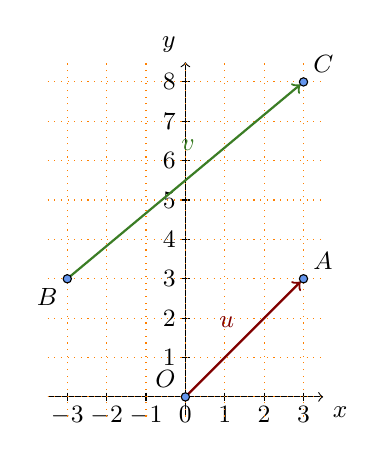
\begin{tikzpicture}[x=5mm,y=5mm, font=\small]

  \begin{scope}[->]
    \draw (-3.5,0) -- (3.5,0) node [below right] {$x$};
    \draw (0,-.5) -- (0,8.5) node[above left] {$y$};
  \end{scope}

  \foreach \x in {-3,-2, ..., 3}{
    \node[below] at (\x, 0) {$\x$};
    \draw (\x,1.5pt) -- (\x,-1.5pt);}
  \foreach \y in {1, 2, ..., 8}{
    \node[left] at (0, \y) {$\y$};
    \draw (1.5pt,\y) -- (-1.5pt,\y);}
  \draw [dotted, orange, step=1](-3.5,-.5) grid (3.5,8.5);

  \begin{scope}[thick, ->,shorten >=1.5pt]
	\draw[Maroon] (0,0) node[above left] at (1.5,1.5) {$u$} -- (3,3);  
	\draw[OliveGreen](-3,3) node[above left] at (.5,6) {$v$}-- (3,8);
      \end{scope}
 
\begin{scope}[fill=CornflowerBlue, draw=black]
\filldraw (0,0) circle (1.5pt)node [above left]{$O$};
\filldraw (3,3) circle (1.5pt)node [above right]{$A$};
\filldraw (-3,3) circle (1.5pt)node [below left]{$B$};
\filldraw (3,8) circle (1.5pt) node [above right]{$C$};
\end{scope}

\end{tikzpicture}
\end{center}
\end{esercizio}
\end{multicols}

\begin{esercizio}
\label{ese:vett.5}
Determinate le componenti del vettore~$\vec{w}=2 \cdot \vec{v}$ 
essendo~$\vec{v}(\frac {3}{2};-2)$ verificate che~$\vec{w}$ e~$\vec{v}$ hanno 
stessa direzione
e~$|\vec{w}|=2 \cdot |\vec{v}|$
\end{esercizio}

\begin{esercizio}
\label{ese:vett.6}
Verificate che~$\frac {3}{2} \cdot (\vec{x}+\vec{y})=\frac {3}{2}\vec{x}+\frac 
{3}{2}\vec{y}$ essendo~$\vec{x}(-\frac {5}{4};1)$ e~$\vec{y}(4;-1)$
\end{esercizio}

\begin{esercizio}
\label{ese:vett.7}
Dati i due vettori~$\vec{u}$ e~$\vec{v}$ di cui si conoscono i moduli e 
l'angolo $\alpha$ che essi formano, disegna i vettori, 
la loro somma e la loro differenza e 
calcola il modulo di~$\vec{u} + \vec{v}$ e di~$\vec{u} - \vec{v}$.
\begin{enumeratea}
\item $u=2; \quad v=4; \quad \alpha=60\grado$ 
 \hfill $\left[\lvert\vec{u} + \vec{v} \rvert \approx 6,08\right]$
\item $u=3; \quad v=5; \quad \alpha=120\grado$ 
 \hfill $\left[\lvert\vec{u} + \vec{v} \rvert \approx 4,35\right]$
\item $u=8; \quad v=4; \quad \alpha=90\grado$ 
 \hfill $\left[\lvert\vec{u} + \vec{v} \rvert \approx 8,92\right]$
\item $u=9; \quad v=6; \quad \alpha=150\grado$ 
 \hfill $\left[\lvert\vec{u} + \vec{v} \rvert \approx 4,84\right]$
\end{enumeratea}
\end{esercizio}

\begin{esercizio}
\label{ese:vett.8}
Dati i due vettori~$\vec{u}$ e~$\vec{v}$ di cui si conoscono i moduli e 
l'angolo $\alpha$ che essi formano, 
calcola il prodotto scalare~$\vec{u} \cdot \vec{v}$.
\begin{enumeratea}
\item $u=2; \quad v=4; \quad \alpha=60\grado$ 
 \hfill $\left[\vec{u} \cdot \vec{v} \approx 4\right]$
\item $u=3; \quad v=5; \quad \alpha=120\grado$ 
 \hfill $\left[\vec{u} \cdot \vec{v} \approx -7,5\right]$
\item $u=8; \quad v=4; \quad \alpha=90\grado$ 
 \hfill $\left[\vec{u} \cdot \vec{v} \approx 0\right]$
\item $u=9; \quad v=6; \quad \alpha=150\grado$ 
 \hfill $\left[\vec{u} \cdot \vec{v} \approx -46,7\right]$
\end{enumeratea}
\end{esercizio}

\begin{esercizio}
\label{ese:vett.9}
Dati i due vettori~$\vec{u}$ e~$\vec{v}$ di cui si conoscono i moduli e 
l'angolo $\alpha$ che essi formano, 
calcola il modulo del prodotto vettoriale~$\vec{u} \times \vec{v}$.
\begin{enumeratea}
\item $u=2; \quad v=4; \quad \alpha=60\grado$ 
 \hfill $\left[\lvert\vec{u} \times \vec{v}\rvert \approx 6,93\right]$
\item $u=3; \quad v=5; \quad \alpha=120\grado$ 
 \hfill $\left[\lvert\vec{u} \times \vec{v}\rvert \approx 12,99\right]$
\item $u=8; \quad v=4; \quad \alpha=90\grado$ 
 \hfill $\left[\lvert\vec{u} \times \vec{v}\rvert \approx 27\right]$
\item $u=12; \quad v=6; \quad \alpha=45\grado$ 
 \hfill $\left[\lvert\vec{u} \times \vec{v}\rvert \approx 50,91\right]$
\end{enumeratea}
\end{esercizio}

% \newpage
% \subsubsection*{F.3 - Dipendenza e indipendenza lineare}
% \begin{esercizio}
% \label{ese:vett.7}
% Completate le scritture:
% \begin{multicols}{2}
% \begin{enumeratea}
% \item $\vec{v}(-\sqrt{2};\frac {5}{4})=\ldots \cdot \vec{i}+\ldots \cdot 
% \vec{j}$
% \item $\vec{u}(1;-1)=\ldots \cdot \vec{i}+\ldots \cdot \vec{j}$
% \item $\vec{h}(\ldots;\ldots)=\frac {\sqrt{3}}{3} \cdot \vec{i}-9 \cdot 
% \vec{j}$
% \item $\vec{z}(\ldots;\ldots)=\frac {3 \sqrt{5}}{3} \cdot \vec{i}$
% \end{enumeratea}
% \end{multicols}
% \end{esercizio}
% 
% \begin{esercizio}
% \label{ese:vett.8}
% \begin{multicols}{2}
%  Dati i vettori della figura, applicate il metodo geometrico per determinare i 
% vettori che permettono di scrivere~$\vec{w}$ come combinazione lineare degli 
% altri due.
% Riprendete questi stessi vettori e determinate i vettori che permettono di 
% scrivere~$\vec{v}$ come combinazione lineare degli altri due. Riprendete questi 
% stessi
% vettori e determinate i vettori che permettono di scrivere~$\vec{u}$ come 
% combinazione lineare degli altri due.
% \begin{center}
% % (c) 2012 Dimitrios Vrettos - d.vrettos@gmail.com

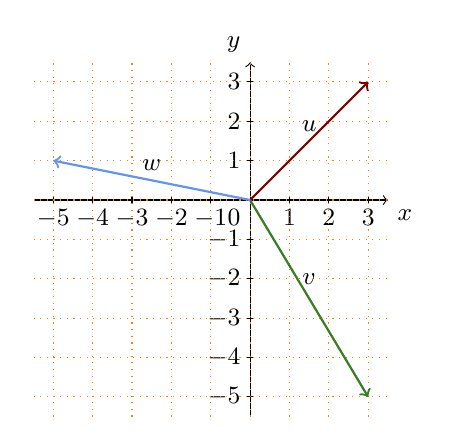
\begin{tikzpicture}[x=5mm,y=5mm, font=\small]

  \begin{scope}[->]
    \draw (-5.5,0) -- (3.5,0) node [below right] {$x$};
    \draw (0,-5.5) -- (0,3.5) node[above left] {$y$};
  \end{scope}

  \foreach \x/\xtext in {-5/-5,-4/-4,-3/-3,-2/-2,-1/-1,1/1,2/2,3/3}{
    \node[below] at (\x,0) {$\xtext$};
    \draw (\x,1.5pt) -- (\x,-1.5pt);}
  \foreach \y/\ytext in {-5/-5,-4/-4,-3/-3,-2/-2,-1/-1,1/1,2/2,3/3}{
    \node[left] at (0,\y) {$\ytext$};
    \draw (1.5pt,\y) -- (-1.5pt,\y);}
  \node[below left] at (0,0) {$0$};

  \begin{scope}[dotted, orange, step=5mm]
    \draw (-5.5,-5.5) grid (3.5,3.5);
  \end{scope}

  \begin{scope}[thick, ->]
	\draw[Maroon] (0,0) -- (3,3);  
	\draw[OliveGreen](0,0) -- (3,-5);
	\draw[CornflowerBlue] (0,0) -- (-5,1);
      \end{scope}
 
\node[above] at (1.5,1.5) {$u$};
\node[above] at (1.5,-2.4) {$v$};
\node[above] at (-2.5,.5) {$w$};
\end{tikzpicture}
% \end{center}
% \end{multicols}
% \end{esercizio}
% 
% \begin{esercizio}
% \label{ese:vett.9}
% I vettori dell'esercizio precedente sono linearmente dipendenti?
% \end{esercizio}
% 
% \begin{esercizio}
% \label{ese:vett.10}
% Spiegate perché i tre vettori~$\vec{v}(1;2)$, $\vec{u}(3;1)$ 
% e~$\vec{w}(-3;-6)$ sono linearmente dipendenti.
% \end{esercizio}
% 
